\documentclass{article}
\usepackage[final]{neurips_2025}
\usepackage{graphicx}
\graphicspath{{figures/}}
\begin{document}
% A made-up paper, for fig-check's example: three figures as a paper might have them.
\begin{figure}
  \centering
  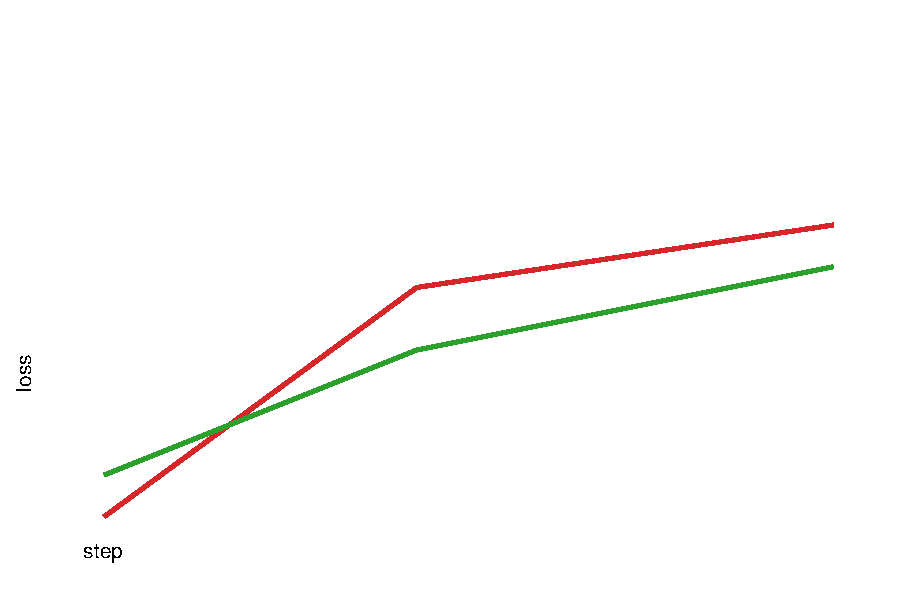
\includegraphics[width=0.48\linewidth]{loss}
  \caption{Training loss: drawn 6 inches wide with 10 pt labels, printed at less than half that size, in red and green.}
\end{figure}
\begin{figure}
  \centering
  
\includegraphics[width=\linewidth]{samples}
  \caption{Samples: a 640-pixel-wide image stretched over the text width.}
\end{figure}
\begin{figure}
  \centering
  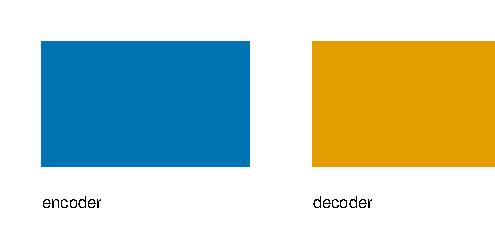
\includegraphics[width=0.6\linewidth]{method}
  \caption{The method: drawn at the size it prints, in blue and orange.}
\end{figure}
\end{document}
